\chapter{Funktioner af flere variable og gradienter}
\label{chap:ch11}

I det foregående kapitel så vi på den afledede som et værktøj til at måle ændringshastigheden for en funktion af én variabel. Geometrisk svarede det til at finde hældningen af en kurve i et punkt. Mange systemer i den virkelige verden afhænger imidlertid af flere faktorer. Et flys brændstoføkonomi afhænger både af dets hastighed og dets flyvehøjde. En maskinlæringsmodels ydeevne er en funktion af tusinder eller endda millioner af parametre. For at kunne håndtere disse komplekse sammenhænge må vi udvide vores forståelse af differentialregning til flere dimensioner.

Det fører os fra den enkle bane langs en kurve til det vidtstrakte terræn på en flade. Forestil dig igen vores vandrer, men nu stående i en bjergkæde. »Hældningen« er ikke længere et enkelt tal; den afhænger helt af, hvilken retning vandreren vælger at vende. Peger man lige op ad bjerget, finder man den stejleste vej, mens man får en helt vandret vej, hvis man vender sig langs bjergets højdekurve. Det matematiske værktøj, der indfanger denne flerdimensionale hældning, er \textbf{gradienten}.


\section{Funktioner af flere variable}

Vi udvider nu vores perspektiv fra funktioner af én variabel, \(f(x)\), til funktioner af to eller flere variable. For enkelhedens skyld fokuserer vi på funktioner af to variable, som skrives \(z = f(x, y)\). Den væsentligste forskel er altså, at vi i stedet for at afbilde værdier af én variabel over i værdier af en anden variabel afbilder ordnede par af variable over i en anden variabel.

\begin{definition}[Funktion af to variable]
En \emph{funktion af to variable} er en regel, der til hvert ordnet par \((x, y)\) i en mængde \(D \subseteq \mathbb{R}^2\) knytter et entydigt reelt tal \(z\), som vi skriver \(z = f(x, y)\). Mængden \(D\) kaldes \emph{definitionsmængden} for \(f\).

\emph{Værdimængden} for \(f\) er mængden af alle reelle tal \(z\), for hvilke der findes mindst ét \((x, y) \in D\), så \(f(x, y) = z\), hvilket er illustreret i \autoref{fig:ch11-domain-range}.
\end{definition}

\begin{figure}[htbp]
    \centering
    \resizebox{0.5\textwidth}{!}{% Danish drawing of a function of two variables mapping a point of the
% domain (a region in the plane) to a number z in the range.
\begin{tikzpicture}[font=\small]
  \fill[mseViaBlue!45, draw=mseViaBlue!70!black]
    plot[smooth cycle, tension=0.8] coordinates {(0,1.6) (1.6,2.3) (3.5,2.4) (3.3,0.9) (3.4,-0.4) (2.2,-1.2) (0.4,-0.6) (-0.6,0.6)};
  \fill[black] (1.4,0.9) circle (2.2pt);
  \node[anchor=north] at (1.4,0.75) {$(x, y)$};
  \draw[mseViaBlue!60!black, thick] (4.3,0.2) -- (8.3,0.2);
  \fill[black] (6.3,0.2) circle (2.2pt);
  \node[anchor=north] at (6.3,0.05) {$z$};
  \draw[-{Stealth[length=7pt]}, very thick, red!70!black] (1.6,1.05) to[out=40, in=120] (6.15,0.35);
  \node at (3.9,2.05) {$f$};
  \node[font=\bfseries] at (1.4,-1.9) {Definitionsmængde};
  \node[font=\bfseries] at (6.3,-1.9) {Værdimængde};
\end{tikzpicture}
}
    \caption{Definitionsmængden for en funktion af to variable består af ordnede par \((x, y)\).}
    \label{fig:ch11-domain-range}
\end{figure}


\begin{example}
    Bestem definitionsmængden og værdimængden for funktionen \(f(x, y) = \sqrt{9 - x^2 - y^2}\).
\end{example}


\begin{figure}
    \centering
    \includegraphics[width=0.5\linewidth]{domain.png}
    \caption{Definitionsmængden for funktionen \(f(x, y)=\sqrt{9-x^2-y^2}\) er en lukket cirkelskive med radius 3.}
    \label{fig:ch11-domain}
\end{figure}

\begin{solution}
    For at bestemme definitionsmængden kræver vi, at udtrykket under kvadratroden er ikke-negativt:
    \[
        9 - x^2 - y^2 \geq 0.
    \]
    Omskrivning giver uligheden
    \[
        x^2 + y^2 \leq 9.
    \]
    Definitionsmængden for \(f\) er derfor den lukkede cirkelskive med radius \(3\) og centrum i origo, som er illustreret i \autoref{fig:ch11-domain}, og som eksplicit er givet ved
    \[
        \operatorname{Dom}(f)
        = \{(x,y) \in \mathbb{R}^2 \mid x^2 + y^2 \leq 9\}.
    \]

    For at bestemme værdimængden bemærker vi, at vi for ethvert punkt \((x,y)\) i definitionsmængden har
    \[
        0 \leq x^2 + y^2 \leq 9,
    \]
    så
    \[
        0 \leq 9 - x^2 - y^2 \leq 9.
    \]
    Ved at tage kvadratroden (og huske, at kvadratroden altid er ikke-negativ) får vi
    \[
        0 \leq f(x,y) = \sqrt{9 - x^2 - y^2} \leq 3.
    \]

    Begge endepunkter i dette interval antages:  
    \begin{itemize}
        \item \(f(x,y) = 3\) i centrum \((0,0)\),
        \item \(f(x,y) = 0\) på randcirklen \(x^2 + y^2 = 9\).
    \end{itemize}

    Værdimængden for \(f\) er altså det lukkede interval
    \[
        \operatorname{Ran}(f) = \{ z \in \mathbb{R} \mid 0 \leq z \leq 3 \} = [0,3].
    \]
\end{solution}

Mens grafen for \(f(x)\) er en kurve i en 2D-plan, er grafen for \(f(x, y)\) en \textbf{flade} i 3D-rummet. Når vi tegner grafen for en funktion af to variable \(z = f(x,y)\), tildeles hvert punkt \((x,y)\) i definitionsmængden en højde \(z\), hvilket giver et ordnet tripel \((x,y,z)\). Samlingen af alle sådanne tripler danner en \emph{flade} i det tredimensionale rum. Man kan forestille sig, at \(xy\)-planen ligger vandret, og at værdien af \(z\) afsættes lodret over (eller under) hvert punkt \((x,y)\). 


\begin{definition}[Niveaukurve og konturkort]
En \textbf{niveaukurve} for en funktion \(f(x, y)\) er mængden af alle punkter \((x, y)\) i inputplanen, hvor funktionen har en konstant værdi, dvs. \(f(x, y) = c\) for en konstant \(c\).

En samling af niveaukurver for forskellige værdier af \(c\) udgør et \textbf{konturkort}.
\end{definition}


\begin{figure}[htbp]
    \caption{Konturkort: (a) et 3D-plot af en flade med niveaukurver projiceret ned på $xy$-planen og (b) et topografisk kort med niveaukurver.}
    \centering
    \begin{subfigure}[based]{0.48\textwidth}
        \centering
        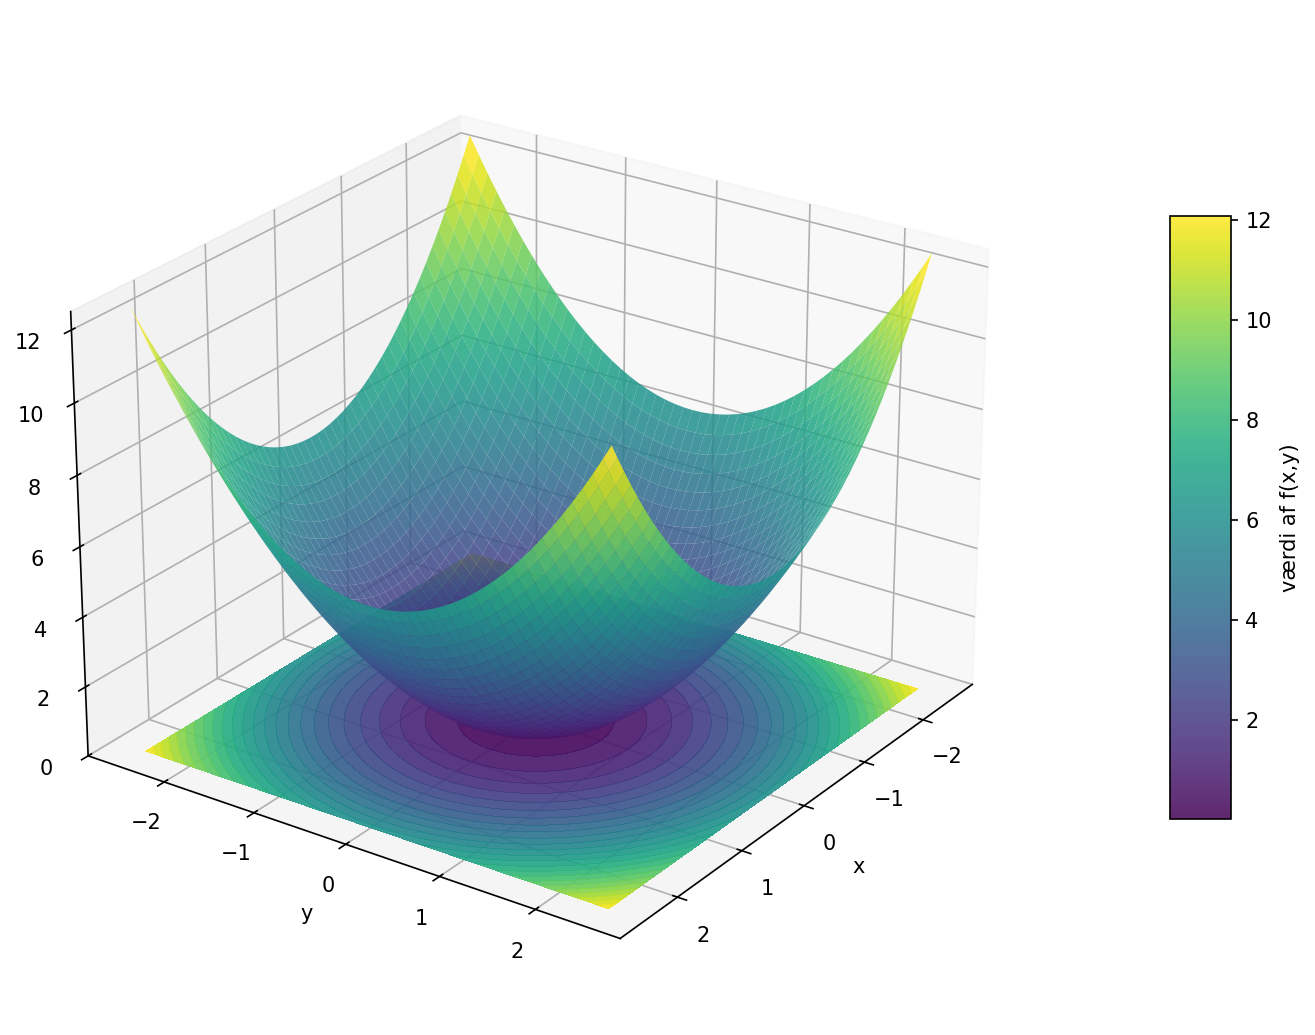
\includegraphics[width=\textwidth]{figure/da/contour_da.png}
        \caption{Fladen $z = x^2 + y^2$ med niveaukurver projiceret ned på $xy$-planen. Hver niveaukurve svarer til en konstant funktionsværdi og illustrerer, hvordan niveaukurver opstår som vandrette snit gennem fladen.}
        \label{fig:ch11-3d-contour-surface}
    \end{subfigure}
    \hfill
    \begin{subfigure}[c]{0.48\textwidth}
        \centering
        \DaTopographicMap{width=\textwidth}
        \caption{Et topografisk kort over et bakket terræn.}
        \label{fig:ch11-topographic-map}
    \end{subfigure}
\end{figure}

På et geografisk kort repræsenterer disse kurver linjer med konstant højde over havet. På vores funktionsflade repræsenterer de kurver med konstant »højde« \(z\). \autoref{fig:ch11-3d-contour-surface} viser fladen \(z = x^2 + y^2\) med niveaukurver projiceret ned på \(xy\)-planen. Hver niveaukurve svarer til en konstant funktionsværdi og illustrerer, hvordan niveaukurver opstår som vandrette snit gennem fladen. \autoref{fig:ch11-topographic-map} viser et topografisk kort over et bakket terræn. Niveaukurver er ikke begrænset til simple funktioner; de kan også repræsentere langt mere komplicerede flader.


\section{Partielle afledede og gradienten}
Hvordan måler vi ændringshastigheden for en funktion af flere variable? Da hældningen afhænger af retningen, kan vi begynde med de simpleste retninger: parallelt med koordinatakserne. Det fører til begrebet \textbf{partiel afledet}.

\subsection*{Partielle afledede}

For en funktion \(z = f(x,y)\) undersøger vi, hvordan fladen ændrer sig, ved at lade den ene variabel variere, mens den anden holdes fast. De ændringshastigheder, vi får, er de \emph{partielle afledede} af \(f\). Den partielle afledede med hensyn til \(x\) beregnes ved at betragte \(y\) som en konstant og differentiere med hensyn til \(x\); den afledede med hensyn til \(y\) findes på tilsvarende måde. Disse to størrelser, \(\partial z/\partial x\) og \(\partial z/\partial y\), beskriver, hvor stejlt fladen stiger eller falder i koordinatretningerne.

Geometrisk repræsenterer \( \frac{\partial f}{\partial x} \) i et punkt \((a, b)\) fladens hældning i x-aksens retning, og \( \frac{\partial f}{\partial y} \) repræsenterer fladens hældning i y-aksens retning.


\begin{definition}[Partielle afledede]
Den \textbf{partielle afledede} af \( f(x, y) \) med hensyn til \( x \), betegnet \( \frac{\partial f}{\partial x} \) eller \( f_x \), er
$$
\frac{\partial f}{\partial x} = \lim_{h \to 0} \frac{f(x+h, y) - f(x, y)}{h}
$$
Den \textbf{partielle afledede} med hensyn til \( y \), betegnet \( \frac{\partial f}{\partial y} \) eller \( f_y \), er
$$
\frac{\partial f}{\partial y} = \lim_{h \to 0} \frac{f(x, y+h) - f(x, y)}{h}
$$
\end{definition}

\begin{example}
    Se på funktionen 
    \[
        f(x,y) = x^{2} + 2y^{2}.
    \]
    Vi beregner dens partielle afledede ved at differentiere med hensyn til den ene variabel, mens den anden holdes konstant.

    \textbf{Partiel afledet med hensyn til \(x\).}

    Betragt \(y\) som en konstant, og differentiér som ved funktioner af én variabel:
    \[
        \frac{\partial}{\partial x}(x^{2} + 2y^{2}) 
        = 2x.
    \]

    Geometrisk svarer det til at skære fladen \(z=f(x,y)\) med en plan \(y=\text{konstant}\), hvilket giver parablen \(z=x^{2}+\text{konstant}\). Værdien \(2x\) er hældningen af denne parabel i det valgte punkt.

    \textbf{Partiel afledet med hensyn til \(y\).} 

    Betragt nu \(x\) som konstant:
    \[
        \frac{\partial}{\partial y}(x^{2} + 2y^{2})
        = 4y.
    \]

    Dette repræsenterer hældningen af det tværsnit, man får ved at skære fladen med en plan \(x=\text{konstant}\).

\end{example}

\begin{example}
    Bestem de partielle afledede af \( f(x, y) = 3x^2 + 2xy^3 + 5y \).
\end{example}

\begin{solution}
    
For at bestemme \( \frac{\partial f}{\partial x} \) betragter vi \( y \) som en konstant:
\[
\frac{\partial f}{\partial x} = \frac{\partial}{\partial x}(3x^2) + \frac{\partial}{\partial x}(2xy^3) + \frac{\partial}{\partial x}(5y) = 6x + 2y^3 + 0 = 6x + 2y^3
\]
For at bestemme \( \frac{\partial f}{\partial y} \) betragter vi \( x \) som en konstant:
\[
\frac{\partial f}{\partial y} = \frac{\partial}{\partial y}(3x^2) + \frac{\partial}{\partial y}(2xy^3) + \frac{\partial}{\partial y}(5y) = 0 + 2x(3y^2) + 5 = 6xy^2 + 5
\]
\end{solution}

\subsection*{Gradientvektoren}

De partielle afledede giver os ændringshastigheden i to bestemte retninger. \textbf{Gradienten} samler denne information i én vektor, der peger i retningen med den \emph{stejleste} ændringshastighed.\footnote{Denne egenskab bevises formelt ved hjælp af begrebet \textit{retningsafledet}, som måler ændringshastigheden i en vilkårlig retning.} Ordet »gradient« betegner i matematik en vektor, der angiver både retningen og stejlheden af stigningen for en funktion af flere variable:

$$
\nabla f(x, y) = \left\langle \frac{\partial f}{\partial x},\ \frac{\partial f}{\partial y} \right\rangle
= 
\begin{bmatrix}
    \frac{\partial f}{\partial x} \\
    \frac{\partial f}{\partial y}
\end{bmatrix}
$$

Symbolet $\nabla$ kaldes \textbf{nabla}- eller \textbf{del}-operatoren.

\begin{definition}[Gradienten]
\textbf{Gradienten} af en funktion \( f(x, y) \), betegnet \( \nabla f \), er den vektorfunktion, der er defineret ved:

$$
\nabla f(x, y) = \left\langle \frac{\partial f}{\partial x}, \frac{\partial f}{\partial y} \right\rangle = \frac{\partial f}{\partial x} \mathbf{i} + \frac{\partial f}{\partial y} \mathbf{j}
$$

\end{definition}

Gradienten er det flerdimensionale sidestykke til den første afledede. Den har to afgørende geometriske egenskaber:
\begin{enumerate}
    \item \textbf{Retning for stejleste stigning:} I et punkt, hvor \(\nabla f(x,y)\neq\vect{0}\), angiver enhedsvektoren $\nabla f/\lVert\nabla f\rVert$ den retning, hvor \(f\) vokser hurtigst.
    \item \textbf{Vinkelret på niveaukurver:} I et regulært punkt, hvor \(\nabla f(x,y)\neq\vect{0}\), er gradienten ortogonal (vinkelret) på niveaukurven gennem \((x,y)\).
\end{enumerate}

Begge egenskaber er yderst nyttige. Den første fortæller os, at gradienten peger i retningen for stejleste stigning, mens den anden forklarer, at denne retning er vinkelret på niveaukurverne. For at komme hurtigst muligt op ad bakke skal man derfor gå i gradientens retning; for at komme hurtigst muligt ned ad bakke skal man gå i den modsatte retning, dvs. langs den negative gradient.

\begin{figure}[htbp]
    \caption{To perspektiver på funktionen \( f(x, y) = 3x^2 + 2xy^3 + 5y \). 3D-billedet (a) viser selve fladen, mens 2D-billedet (b) viser det konturkort, vi bruger i analysen. De røde gradientvektorer peger i retningen for stejleste stigning og er altid vinkelrette på niveaukurverne.}
    \centering
    % Subfigure for the 3D plot
    \begin{subfigure}[b]{0.55\textwidth}
        \centering
        \includegraphics[width=\textwidth]{surface_with_projected_gradients.png}
        \caption{Et 3D-billede af fladen \(z = f(x, y)\) med dens gradientfelt projiceret nedenunder.}
        \label{fig:ch11-3d-view}
    \end{subfigure}
    \hfill % Adds a little space between the figures
    % Subfigure for the 2D plot
    \begin{subfigure}[b]{0.41\textwidth}
        \centering
        \includegraphics[width=\textwidth]{contour_with_gradients.png}
        \caption{Et 2D-billede set ovenfra, der viser konturkortet og gradientfeltet.}
        \label{fig:ch11-2d-view}
    \end{subfigure}

    \label{fig:ch11-side-by-side}
\end{figure}

For fuldt ud at forstå gradientens geometriske betydning er det nyttigt at se den fra to forskellige perspektiver, som vist i \autoref{fig:ch11-side-by-side}. Figuren viser den samme funktion, \( f(x, y) = 3x^2 + 2xy^3 + 5y \), på to måder: som en tredimensional flade og som et todimensionalt konturkort.

Til venstre, i \autoref{fig:ch11-3d-view}, ser vi funktionen som et landskab. Fladens højde i ethvert punkt \((x, y)\) svarer til værdien af \(z = f(x, y)\). Under fladen har vi projiceret dens konturkort sammen med dens gradientfelt, som er vist med røde pile. Man kan visuelt følge, hvordan fladens stejlhed i et punkt hænger sammen med pilen lige under det.

Til højre, i \autoref{fig:ch11-2d-view}, har vi det perspektiv, vi oftest arbejder med: et billede af xy-planen set ovenfra. Det er det almindelige konturkort, hvor hver kurve forbinder punkter med samme »højde«. Gradientvektorerne er lagt oven på dette kort.

Ved at sammenligne de to billeder kan vi bekræfte gradientens to grundlæggende egenskaber:

\begin{enumerate}
    \item \textbf{Retning for stejleste stigning:} Se på en vilkårlig rød pil på 2D-kortet. Bemærk, at den altid peger fra et område med lavere værdier (lysere farver) mod et område med højere værdier (mørkere farver). Pilene viser retningen »op ad bakke«. Det svarer direkte til den stejleste vej, man kan tage op ad fladen i 3D-billedet.
    
    \item \textbf{Vinkelret på niveaukurver:} Se på sammenhængen mellem de røde pile og de hvide niveaukurver i \autoref{fig:ch11-2d-view}. I hvert punkt er gradientvektoren præcis ortogonal (vinkelret) på den niveaukurve, der går gennem punktet. Det giver intuitivt mening: For at bestige en bakke mest effektivt skal man gå vinkelret på de kurver, der har samme højde.
\end{enumerate}

Denne sammenligning side om side bygger bro mellem den fysiske virkelighed i funktionens form og de matematiske værktøjer, vi bruger til at analysere den.

\section{Anvendelser af gradienten}

Gradienten er et af de mest grundlæggende begreber i anvendt matematik med vidtrækkende betydning i fysik, ingeniørvidenskab og datalogi, og den er hjørnestenen i den seneste udvikling inden for maskinlæring og kunstig intelligens.

\subsection*{Optimering og gradientnedstigning}
Husk vores vandrer, der prøver at finde det laveste punkt i en tåget dal. Den mest effektive strategi er altid at gå i retningen for stejleste \emph{fald}. Ud fra gradientens egenskaber ved vi, at denne retning er præcis modsat gradientvektoren, \( -\nabla f \).

Denne enkle idé er grundlaget for algoritmen \textbf{gradientnedstigning}, som er central for træningen af moderne maskinlæringsmodeller. Vandrerens »højde« er modellens fejl (eller tabsfunktion), og »positionen« er mængden af modelparametre. Algoritmen fungerer således:

\vspace{1cm}

\begin{enumerate}
    \item Start i et tilfældigt punkt (et tilfældigt sæt parametre).
    \item Beregn tabsfunktionens gradient i dette punkt.
    \item Tag et lille skridt i den negative gradients retning, \( -\nabla f \).
    \item Gentag, indtil et valgt stopkriterium er opfyldt, fx en lille gradientnorm eller en tilstrækkelig lille ændring i tabet.
\end{enumerate}

Denne iterative proces følger lokale nedstigningsretninger og kan finde brugbare parameterværdier, selv når en funktion har millioner af variable. En lille gradient garanterer ikke i sig selv et lokalt minimum, og for en generel ikke-konveks tabsfunktion kan metoden nærme sig et saddelpunkt eller et lokalt minimum, der ikke er globalt.

\begin{example}

En simpel tabsfunktion er givet ved \( L(w_1, w_2) = w_1^2 + 2w_2^2 \). Hvis vi befinder os i punktet \((w_1, w_2) = (2, 1)\), i hvilken retning skal vi så bevæge os for at mindske tabet hurtigst?
\end{example}
\begin{solution}
Vi skal finde den negative gradients retning, \( -\nabla L \).
Først beregner vi gradienten:
\[
\nabla L = \left\langle \frac{\partial L}{\partial w_1}, \frac{\partial L}{\partial w_2} \right\rangle = \langle 2w_1, 4w_2 \rangle
\]
Dernæst evaluerer vi gradienten i punktet \((2, 1)\):
\[
\nabla L(2, 1) = \langle 2(2), 4(1) \rangle = \langle 4, 4 \rangle
\]
Den negative gradient er en vektor i retningen for stejleste fald:
\[
-\nabla L(2, 1) = \langle -4, -4 \rangle
\]
Den tilsvarende enhedsretning er $\langle-1/\sqrt{2},-1/\sqrt{2}\rangle$. Et skridt i gradientnedstigning er proportionalt med $\langle-4,-4\rangle$, og skridtlængden styres af læringsraten.
\end{solution}

\section{Anvendelse: Træning af en model med gradientnedstigning}

Vi har set, at gradienten, \(\nabla f\), peger i retningen for stejleste stigning, og at dens negative, \(-\nabla f\), peger i retningen for stejleste fald. Dette princip er ikke blot en geometrisk kuriositet; det er motoren bag træningen af de fleste moderne maskinlæringsmodeller. Vi gennemgår nu et komplet, praktisk eksempel: at finde den optimale linje, der passer til et datasæt, ved hjælp af \textbf{lineær regression} og algoritmen \textbf{gradientnedstigning}.

\begin{example}
    Optimering af en simpel lineær regressionsmodel
\end{example}

\begin{solution}
Forestil dig, at vi har et datasæt bestående af \(n\) punkter \((x_i, y_i)\). For eksempel kunne \(x_i\) være størrelsen af et hus og \(y_i\) dets pris. Vores mål er at finde den rette linje, der passer bedst til disse data. Denne proces kaldes lineær regression.

\vspace{1em}
\textbf{Trin 1: Definér modellen}

En ret linje er bestemt ved sit konstantled (\(\beta_0\)) og sin hældning (\(\beta_1\)). For ethvert givet input \(x_i\) forudsiger vores model en værdi, som vi kalder \(\hat{y}_i\), ifølge ligningen:
\[
\hat{y}_i = \beta_0 + \beta_1 x_i
\]
Vores opgave er at finde de optimale værdier af parametrene \(\beta_0\) og \(\beta_1\).

\vspace{1em}
\textbf{Trin 2: Definér tabsfunktionen}

Hvordan ved vi, om en linje »passer godt«? Vi måler dens fejl. For hvert datapunkt er fejlen forskellen mellem den faktiske værdi (\(y_i\)) og den forudsagte værdi (\(\hat{y}_i\)). For at sikre, at fejlene ikke ophæver hinanden, og for at straffe store fejl hårdere, kvadrerer vi disse forskelle. Derefter tager vi gennemsnittet af den kvadrerede fejl over alle \(n\) datapunkter. Det giver os tabsfunktionen \textbf{middelkvadratfejlen} (MSE, af engelsk \emph{mean squared error}), \(L\):
\[
L(\beta_0, \beta_1) = \frac{1}{n} \sum_{i=1}^{n} (y_i - \hat{y}_i)^2 = \frac{1}{n} \sum_{i=1}^{n} (y_i - \beta_0 - \beta_1 x_i)^2
\]
Dette er den centrale ligning. Bemærk, at tabet \(L\) ikke er en funktion af \(x\) eller \(y\) (som er faste datapunkter), men en funktion af modellens parametre, \(\beta_0\) og \(\beta_1\). Det er en konveks andengradsflade: typisk skålformet, selv om den kan have en flad retning, hvis dataene ikke bestemmer begge parametre entydigt. Vores mål er at finde et globalt minimum for denne flade.

\vspace{1em}
\textbf{Trin 3: Beregn tabsfunktionens gradient}

For at finde bunden af tabsfladen med gradientnedstigning skal vi kende retningen for stejleste fald i ethvert punkt. Det kræver, at vi beregner gradienten af \(L\) med hensyn til dens variable, \(\beta_0\) og \(\beta_1\). Gradienten er vektoren af partielle afledede:
\[
\nabla L = \left\langle \frac{\partial L}{\partial \beta_0}, \frac{\partial L}{\partial \beta_1} \right\rangle
\]
Vi finder hver partiel afledet ved hjælp af differentiationsreglerne, især kædereglen.

For \(\frac{\partial L}{\partial \beta_0}\) betragter vi \(\beta_1\) som en konstant og differentierer:
\[
\frac{\partial L}{\partial \beta_0} = \frac{1}{n} \sum_{i=1}^{n} 2(y_i - \beta_0 - \beta_1 x_i) \cdot (-1) = -\frac{2}{n} \sum_{i=1}^{n} (y_i - \beta_0 - \beta_1 x_i)
\]
For \(\frac{\partial L}{\partial \beta_1}\) betragter vi \(\beta_0\) som en konstant og differentierer:
\[
\frac{\partial L}{\partial \beta_1} = \frac{1}{n} \sum_{i=1}^{n} 2(y_i - \beta_0 - \beta_1 x_i) \cdot (-x_i) = -\frac{2}{n} \sum_{i=1}^{n} (y_i - \beta_0 - \beta_1 x_i) x_i
\]
Disse to udtryk giver os komponenterne i gradientvektoren \(\nabla L\) for alle givne værdier af \(\beta_0\) og \(\beta_1\).

\vspace{1em}
\textbf{Trin 4: Algoritmen gradientnedstigning}

Nu har vi alle brikkerne. Algoritmen gradientnedstigning er en iterativ proces:
\begin{enumerate}
    \item Start med et første gæt på \(\beta_0\) og \(\beta_1\) (fx tilfældige værdier).
    \item Beregn gradienten \(\nabla L\) ud fra de aktuelle værdier af \(\beta_0\) og \(\beta_1\).
    \item Opdatér parametrene ved at tage et lille skridt i den \emph{negative} gradients retning.
\end{enumerate}
Dette opdateringstrin er kernen i algoritmen. Vi indfører en lille positiv konstant \(\eta\) (eta), kaldet \textbf{læringsraten}, som styrer størrelsen af vores skridt. Opdateringsreglerne er:
\[
\beta_0 \leftarrow \beta_0 - \eta \frac{\partial L}{\partial \beta_0}
\]
\[
\beta_1 \leftarrow \beta_1 - \eta \frac{\partial L}{\partial \beta_1}
\]
Vi gentager denne proces mange gange. For hvert skridt bevæger parametrene \(\beta_0\) og \(\beta_1\) sig tættere på de værdier, der minimerer tabsfunktionen \(L\), så de reelt »går ned ad bakke« på tabsfladen, indtil de falder til ro i bunden.

Med en mere kompakt vektornotation, hvor \(\boldsymbol{\beta}\) er vektoren \(\langle \beta_0, \beta_1 \rangle\), kan hele opdateringsreglen skrives som:
\[
\boldsymbol{\beta} \leftarrow \boldsymbol{\beta} - \eta \nabla L
\]
Dette ene udtryk indfanger på elegant vis processen med at optimere en maskinlæringsmodel. Det er en direkte og stærk anvendelse af gradienten og viser, hvordan et grundlæggende begreb fra differentialregningen bruges til at løse komplekse problemer fra den virkelige verden. \end{solution}

I dette kapitel har vi udvidet begrebet den afledede til flere variable. Vi begyndte med at se på funktioner af flere variable og partielle afledede og til sidst på gradientvektoren. Gradienten, som er den »fulde« afledede for funktioner af flere variable, beskriver ikke blot ændringshastigheden i alle retninger, men giver også det teoretiske grundlag for effektive optimeringsalgoritmer, der driver moderne teknologi. Derefter anvendte vi gradienten på problemet med at finde den optimale linje, der passer til et datasæt, ved hjælp af lineær regression og algoritmen gradientnedstigning. Dette afslutter kapitlet og dermed denne del af bogen Matematik for softwareingeniører.
